\PassOptionsToPackage{svgnames}{xcolor}
\documentclass[a4paper, 12pt]{article}

\usepackage{hyperref}

\hypersetup{
	colorlinks,
	linkcolor={black},
	citecolor={black},
	urlcolor={black}
}
\usepackage{lmodern}
%\usepackage{geometry}
%\usepackage{layout}
\usepackage{graphicx}
\usepackage{wrapfig}

\title{Artificial Teacher}
\author{Alex Tsvetanov}	

\newcommand{\titleGP}{\begingroup
	\centering
	%\vspace{\baselineskip}
	\rule{\textwidth}{1.6pt}\vspace{-\baselineskip}\vspace{2pt}
	\rule{\textwidth}{0.4pt}\\[\baselineskip]
	
	{\LARGE Artificial teacher}\\[0.2\baselineskip]
	
	\rule{\textwidth}{0.4pt}\vspace{-\baselineskip}\vspace{3.2pt}
	\rule{\textwidth}{1.6pt}\\[\baselineskip]
	\begin{wrapfigure}{r}{0.35\textwidth}
		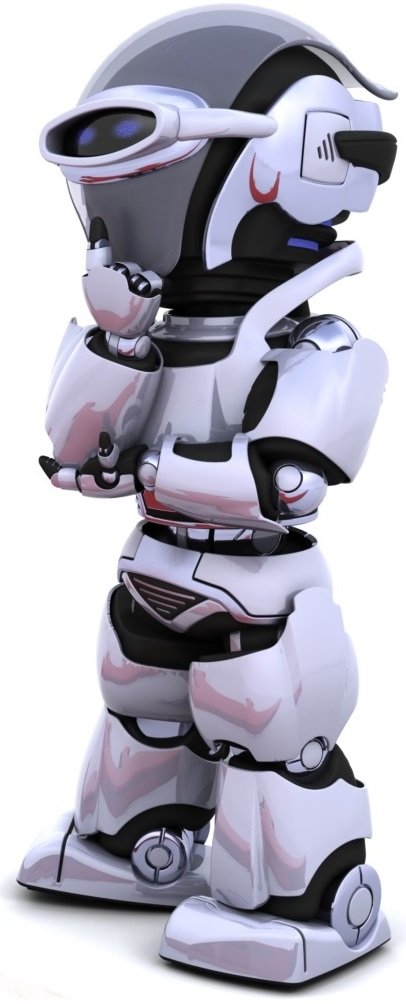
\includegraphics[scale=0.5]{logo.png}
	\end{wrapfigure}
	
	\vspace{50pt}
	{\LARGE Alex Ivanov Tsvetanov\\\par}
	{\itshape \Large High School of Mathematics \\ Sofia, Bulgaria\par}
	
	\vspace{2\baselineskip}
	
	{\scshape \large
		Under the direction of \\
		ch. ace. Emil Kelevedjiev\\\&\\assoc. Zlatogor Minchev\\\par
	}
	\vspace{1cm}
	
	
	\vfill
	
	{\scshape Summer Research School, 2017} \\[0.3\baselineskip]
	{\large Blagoevgrad, Bulgaria }\par
	
	\endgroup}

\usepackage{tcolorbox}
\newenvironment{myblock}[1]{%
	\tcolorbox[beamer,%
	noparskip,breakable,
	colback=LightGreen,colframe=DarkGreen,%
	colbacklower=LimeGreen!75!LightGreen,%
	title=#1]}%
{\endtcolorbox}

\begin{document}

	\titleGP
	\newpage
	
	\tableofcontents
	\newpage
	
	\begin{abstract}
		In fact there are a lot of built-in learning management systems, but there are not any system that combines the newest technologies in education - there are not any system that uses artificial intelligence and virtual reality at once. \\
		\\
		The core aim of our project is to create system that combines these techniques and to build "artificial teacher" that combines best practices in organizing training so that it will be interesting, useful and much easier for the students. The most important part of our project is to fertilize students, showing them that their subjects is not as difficult as sound.\\
		\\		
		Teacher will train student by lessons and different types of exercises which will include theoretical part, but will mostly be oriented practically. 
	\end{abstract}
	\vspace{1cm}
	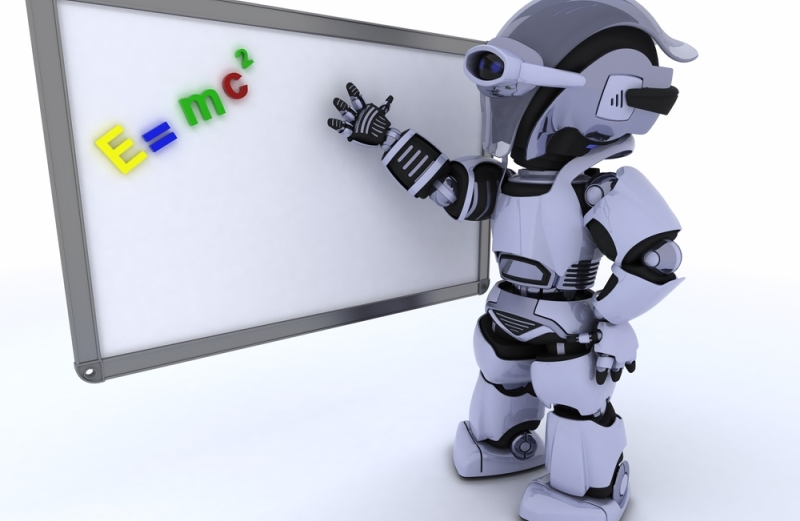
\includegraphics[width=\textwidth]{./robot-teacher.jpg}
	\newpage
	
	\section{Introduction}
	
	\vspace{1cm}
	\large{
		\begin{myblock}{"Learning management system"}
			It is a software application for the administration, documentation, tracking, reporting and delivery of educational courses or training programs.
		\end{myblock}
		\vspace{1cm}
		\begin{myblock}{"Artificial teacher"}
			It is a system that must teach students by interactive, interesting, useful and much easier way for them. It can be represented as "individual mentor" in specific subject.
		\end{myblock}
		\vspace{1cm}
		There are a lot of built-in learning management systems, but there are not any system that combines artificial intelligence and virtual reality at once. \\
		\\
		The aim of our project is to create system that to build "artificial teacher" by following newest technologies and best practices in organizing training so that it will be interactive, interesting, useful and much easier for the students. The most important part of our project is to fertilize students, showing them that their subjects is not as difficult as sound.\\
		\\		
		Teacher will train student by lessons and different types of exercises which will include theoretical part, but will mostly be oriented practically. 
	}
	\section{Implementation}
		Our project is divided by two parts:
		\begin{itemize}
			\item[beauty] Design, which must implement human facial expressions for better sense of reality. 
			\item[intelligence] Application Public Interface that must return material which must be learnt by student
			\item[communication] Live bot chat for all questions during the lesson that "artificial teacher" presents. 
		\end{itemize}
		Each part has a lot of specifics and thus that this project is so hard, but it would give a different view of learning, a more modern look.
		\subsection{Problems}
			\subsubsection{Application Public Interface}
				The most important thing when you develop artificial intelligence is that you must have enough data, which you will use for training of the AI. \\ \\
				Current training data is only sample data and it is not so formal, but is enough for start.
			\subsubsection{Design}
				Design is not ready yet, because it costs a lot of time until we design 3D object and until we implement all human facial expressions. 
			\subsubsection{Communication}
	\section{Techniques}
	\begin{itemize}
		\item C++ for AI in combination with FastCGI++
		\item ...
		\item ...
	\end{itemize}
	\section{Future}
 	\section{Acknowledgments}
 	 	 Special thanks to:
 	 	 \begin{itemize}
 	 	 	\item Zlatogor Minchev for the improvement of the idea
 	 	 	\item Emil Kelevejiev for the improvement of the project
 	 	 \end{itemize}
 	 	 Thanks also to:
 	 	 \begin{itemize}
 	 	 	\item High School Students Institute of Mathematics and Informatics
 	 	 	\item Bulgarian Academy of Sciences
 	 	 	\item Sofia High School of Mathematics
 	 	 \end{itemize}
 	 	 \begin{thebibliography}{99}
 	 	 	\bibitem{gcc}
 	 	 	{\itshape GNU Compiler Collection}.
 	 	 	\texttt{https://gcc.gnu.org/}. \\
 	 	 	Copyright \copyright\  2009 Free Software Foundation, Inc.
 	 	 	\bibitem{mariadb}
 	 	 	{\itshape MariaDB}.
 	 	 	\texttt{https://mariadb.org/}. \\
 	 	 	Copyright \copyright\  2017 MariaDB Foundation
 	 	 	\bibitem{mariadb}
 	 	 	{\itshape MariaDB++}.
 	 	 	\texttt{https://mariadb.org/}. \\
 	 	 	Copyright \copyright\  2017 MariaDB Foundation
 	 	 	\bibitem{latex}
 	 	 	{\itshape \LaTeX}.
 	 	 	\texttt{https://www.latex-project.org/}.
 	 	 \end{thebibliography}
\end{document}
